%\chapter{Bose--Einstein condensate dynamics}
\section{Condensate dynamics}
For steady-state solutions of the Gross--Pitaevskii equation one can examine the properties of a condensate for many different initial conditions, wherein one can make use of Eq.~\ref{eqn:gpe_stationary}. With the background theory outlined in Sections~\ref{sec:superfluid,sec:coldatoms}, I will now discuss manipulations and dynamics of the condensate. Due to phase coherence over all atoms, we can say that any perturbation to the condensate phase will have some effect on all condensed atoms. Direct manipulation of the phase is interesting as the condensate phase encapsulates all quantum behaviour of the system. Secondly, given the phase term is modifiable to any arbitrary values (within the range $\pm \pi$), following Eq.~\ref{eqn:madelung}, one can assume any direct or indirect manipulations of this phase can give rise to interesting dynamics and states.

Given that the condensate velocity determined by Eq.~\ref{eqn:velocity}, it is possible through engineering of the condensate phase, to control the atomic velocity, as given by eq.~\ref{eqn:velocity}. This opens an interesting set of possibilities as control of the phase, and hence velocity, allows for development of a wide range of quantum states and dynamics. Following some form of perturbative manipulation the BEC will evolve in time subject to the applied manipulation. I will discuss some experimentally realistic methods to examine such evolution behaviour, wherein I manipulate various aspects of the Hamiltonian and resulting wavefunction.

Two such manipulations I will focus on will be control of the trapping potential geometry in the Hamiltonian, $V$, as well as direct control of the wavefunction phase, $\theta$. I will begin with a discussion of the former.



\section{Simulating Bose--Einstein condensates}
To verify the model of a Bose--Einstein condensate and the numerical procedures laid out previously, it is instructive to examine the numerical solution of a BEC with that of the Thomas-Fermi profile, as given by Eq.~\ref{eqg:thomasfermi}. The profile and width should be comparable, with the TF solution deviating within the low-density regions. Fig.~\ref{fig:gpe_tf_3} shows a comparison of the two-dimensional profile for both methods, showing good agreement, and hence a well developed numerical procedure.
\begin{figure}\centering
    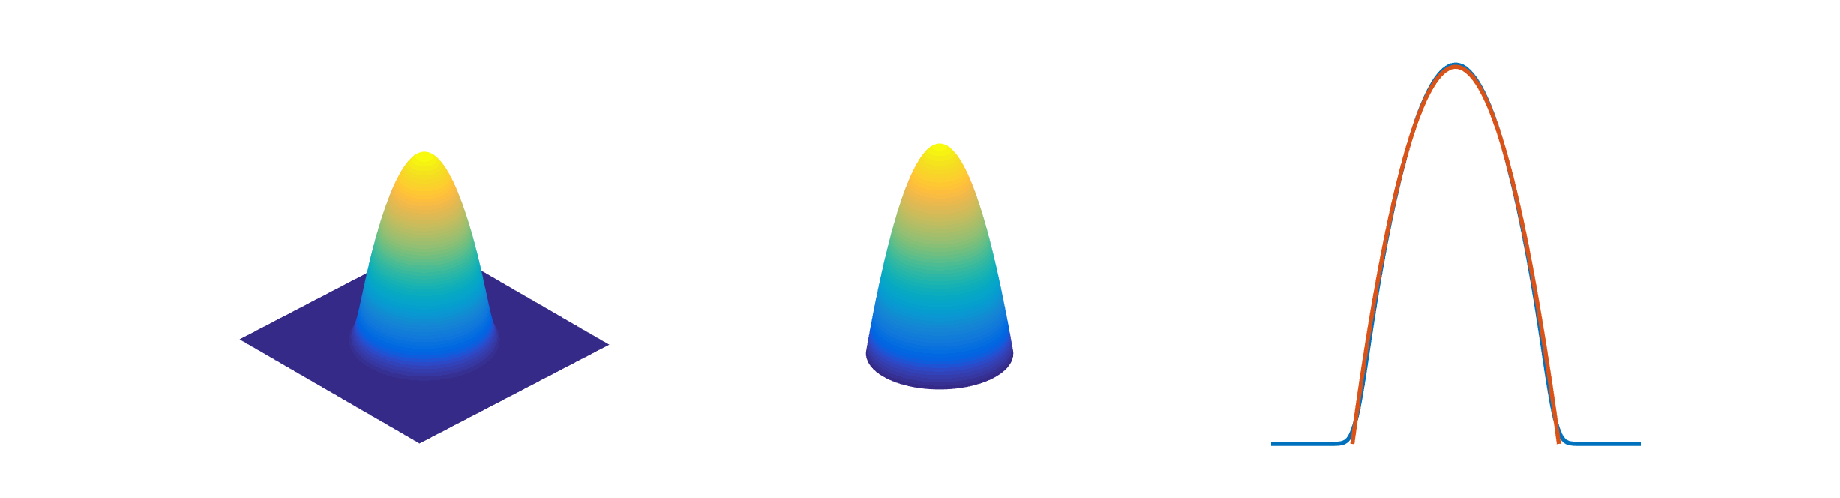
\includegraphics[width=\textwidth,trim=20ex 0ex 20ex 10ex]{Images/ch4_vtx/gpe_tf_3.pdf}
    \caption{The numerical solution (L) and Thomas-Fermi (M) solutions for a two-dimensional condensate of $^{87}$Rb with $N=1\times 10^5$ atoms. The lineplot (R) is a central cut through both profiles showing the close match.}\label{fig:gpe_tf_3}
\end{figure}

While the Thomas--Fermi solution is a close agreement with the numerical solution of the Gross--Pitaevskii equation, this is applicable only in a small number of cases. For more complex problems involving dynamics, the use of Gross--Pitaevskii is required. One such example is that of superfluid vortex dynamics. The numerical generation of a stable set of vortices in a Bose--Einstein condensate is achieved by solving the Gross--Pitaevskii equation Hamiltonian in the frame co-rotating with a time dependent rotating harmonic potential, eq.~\ref{eqn:gpe}. To seed a single vortex in the condensate, the frequency of rotation, $\Omega$, must be higher than the critical rotation frequency $\Omega_C$, as discussed in Sec.~\ref{sec:}, and evolved in imaginary time to allow for energetic losses.

%%% Need to fix this


\subsection{Trapping potential control}

Assuming a system is modeled effectively by GPE Eq.~\ref{eqn:gpe}, with Hamiltonian $H = H_0$, allows for a numerically evaluated ground-state with respect to this Hamiltonian. Any change to the Hamiltonian, performed slowly enough (adiabatically) will allow for the wavefunction to follow this change and remain in the groundstate of the new Hamiltonian. However, let us now imagine an abrupt change, $H = H_0 + \xi H_1$. In this scenario, the wavefunction, formerly a stationary state of $H_0$, will no longer remain so in the new Hamiltonian for $\xi > 0$. Any modification of the Hamiltonian in this way can be viewed as a method for changing the phase of the resulting wavefunction, given sufficient evolution time, $t$ following
%\begin{equation}
%    e^{i\phi} \mapsto \exp\left(-i\frac{Ht}{\hbar}\right),
%\end{equation}

\begin{subequations}
\begin{align}
    \Psi_0 &= |\Psi_0|e^{i\theta_0} \\
    \Psi(t) &= \Psi_0 e^{-\frac{i H t}{\hbar}} \\
    \Psi(t) &= |\Psi_0| e^{i\left(\theta_0 - \frac{H t}{\hbar}\right)} \\
    \theta^{'} &= \theta_0 - \frac{H t}{\hbar}
\end{align}
\end{subequations}
wherein I have made use of Eq.~\ref{eqn:madelung}. By modifying the Hamiltonian the resulting components of the wavefunction see a different phase which governs their evolution. One common means to manipulate the Hamiltonian is through the use of optical potentials, which can be adjusted and manipulated through a variety of ways. Given the importance of magneto-optical traps (MOT) in trapping BECs, the inclusion of additional optical fields should be experimentally possible. Optical lattices have become very prolific in BEC experiments, with experimental control being very highly developed. Thus, the creation of optical potentials for condensed atoms is expected to be a widely available experimental technique.

An arbitrary set of optical fields can be given by
\begin{equation}\label{eqn:optfield}
    f_{\textrm{P}} = \displaystyle\sum\limits_{j} \alpha_j e^{\textrm{i}\left(\mathbf{k}_j\cdot\mathbf{r} - \omega t\right)},
\end{equation}
where $j$ is the row index of the individual optical field, $\alpha_j$ is the amplitude of the field, $\mathbf{k}_j$ is the respective wavevector, and $\omega$ is the oscillation frequency of the wave. By careful choice of $\alpha$ and $\mathbf{k}$ any arbitrary potential geometry can be formed through Fourier synthesis. For the purpose of my system this may reduced through several simplifications, resulting in what remains as a realistic system. Given that an explicit time-dependence on the potentials would introduce experimental difficulties, one can assume that for the cases examined herein that the optical fields are time independent (i.e $\omega=0$), and are counter-propagating plane waves. This reduces the summation to a linear combination of cosine terms. Lastly, as I only require the intensity for defining the potential geometry, the corresponding optical potential can be written as
\begin{equation}\label{eqn:vopt}
    V_{\textrm{O}} = \displaystyle\sum\limits_{j} \gamma_j \cos^2 \left(\mathbf{k}_j \mathbf{r}\right),
\end{equation}
where $\gamma$ is the amplitude of the individual potential components. By choosing the values of $\mathbf{k}_j$ to match the lattice vectors of a required lattice geometry, the optical potential may take this form. For the work described herein I restrict the dynamics to two-dimensions. Fig.~\ref{fig:squarelatt} demonstrates this with a square lattice geometry, given by
\begin{equation}\label{eqn:sqlatt}
    \mathbf{k} =
    \begin{bmatrix}
     1 & 0 \\
     0 & 1
    \end{bmatrix} =
    \begin{bmatrix}
     \mathbf{k}_1  \\
     \mathbf{k}_2
    \end{bmatrix}.
\end{equation}

\begin{figure}\centering
    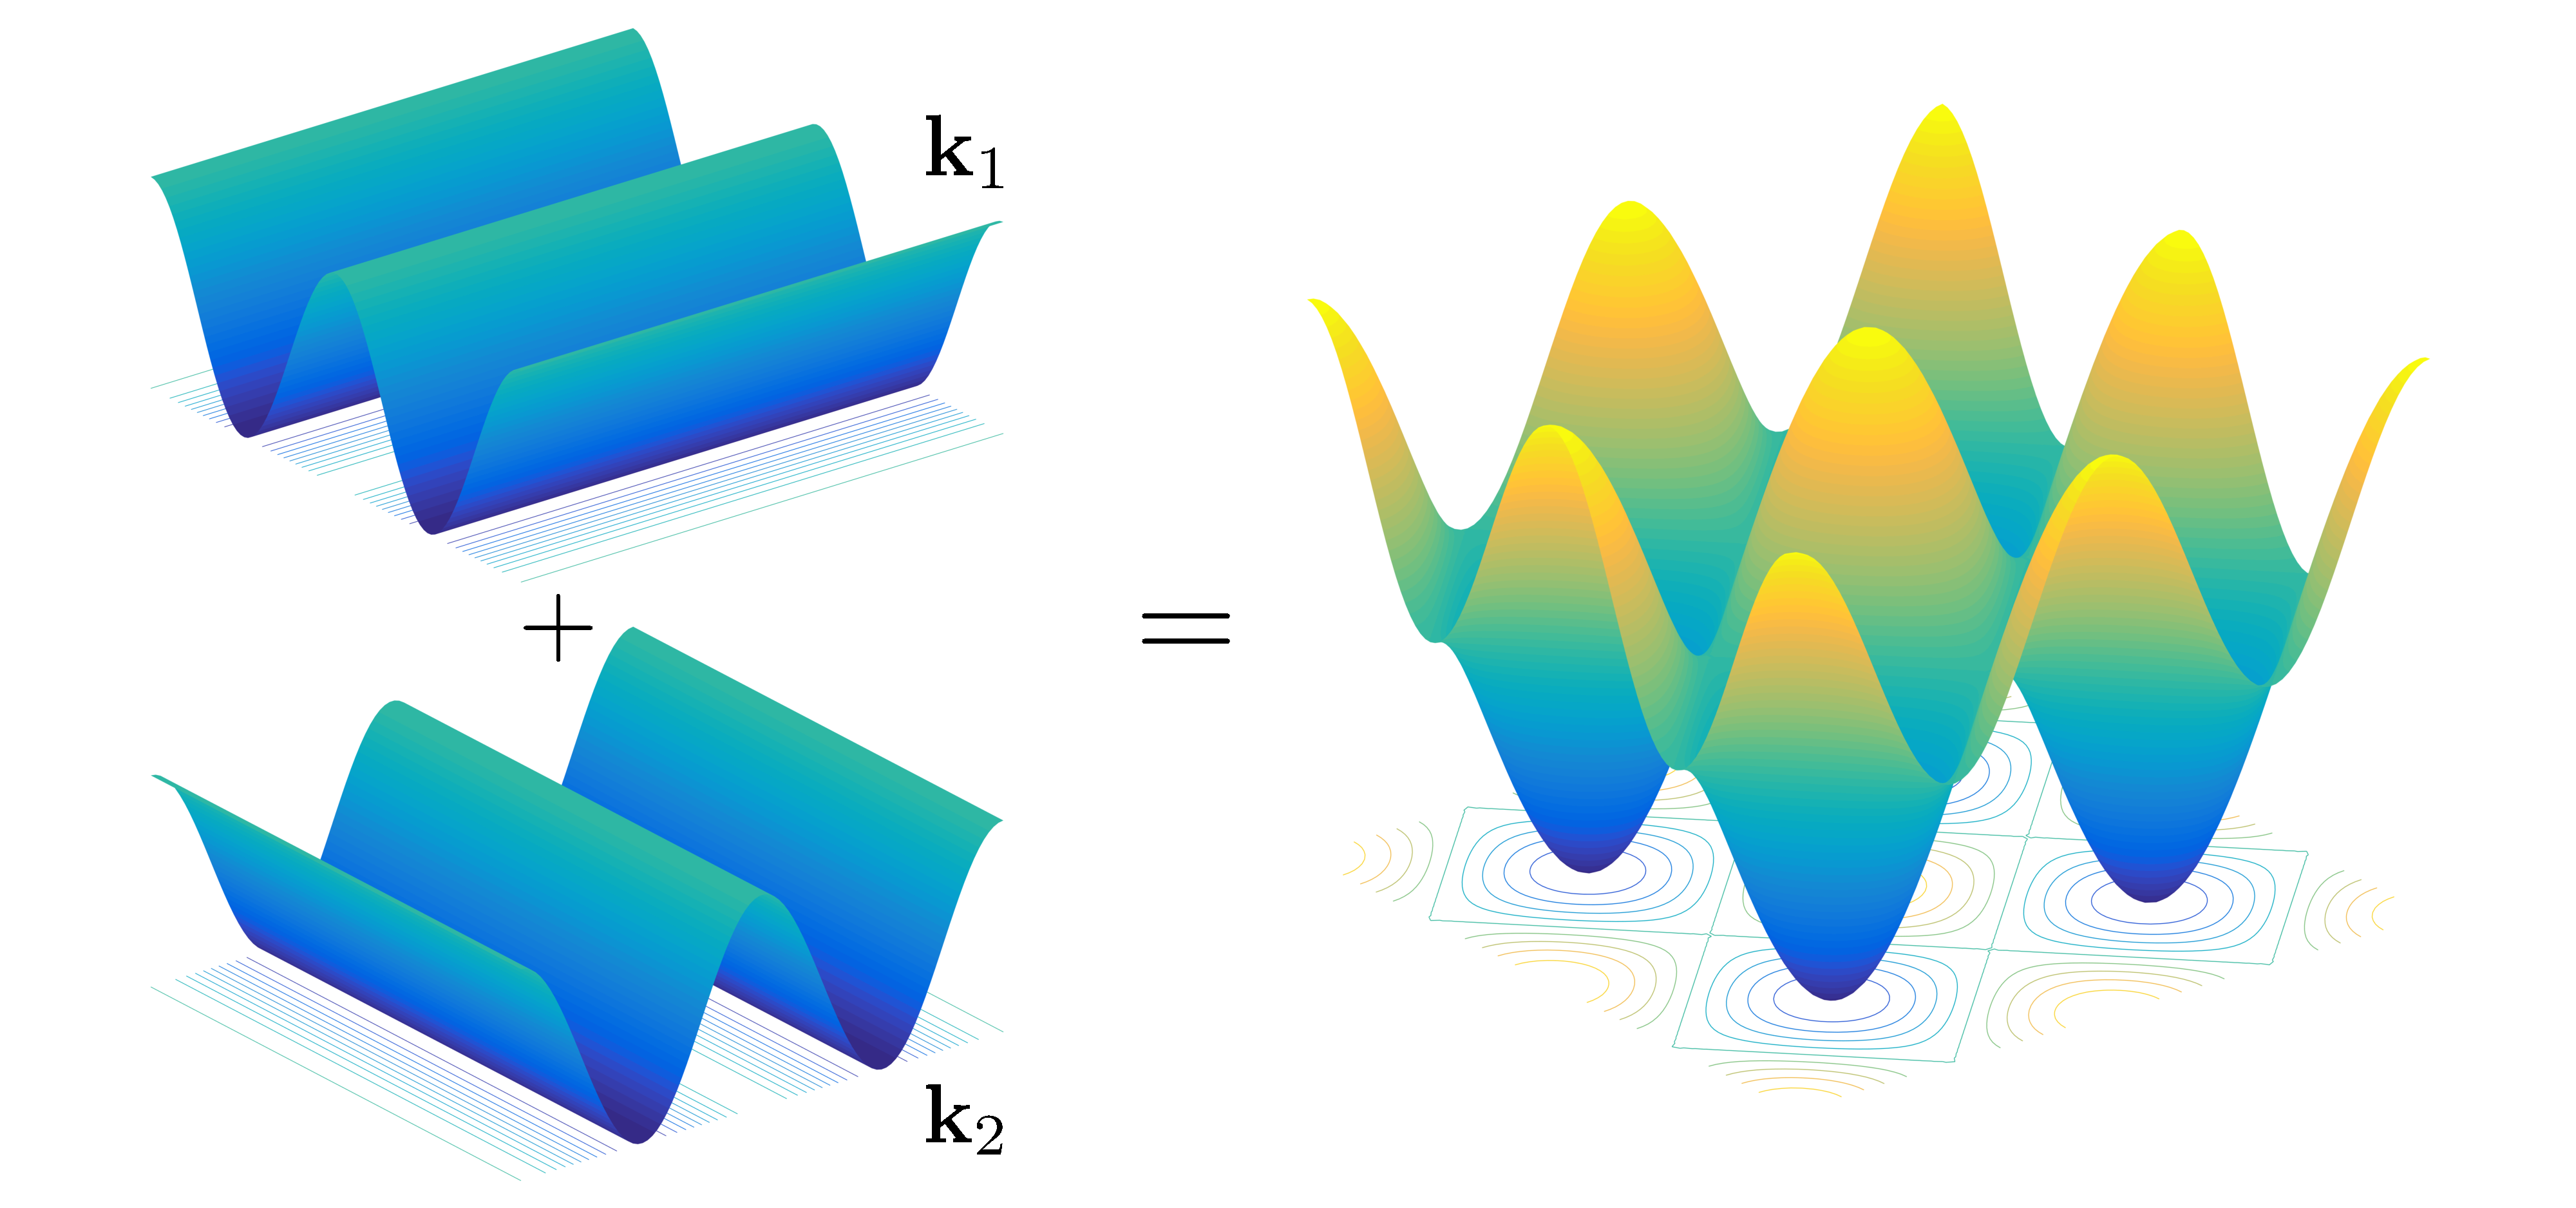
\includegraphics[width=0.55\textwidth]{./Images/ch4_vtx/VOPT/squarelatt}
    \caption{Square lattice generation using two orthogonal propagating laser fields, as defined by Eq.~\ref{eqn:sqlatt}.}\label{fig:cos2xy}
\end{figure}

By setting $H_1 = V_{\textrm{O}}$, the evolution of the condensate following the new additional potential can be controlled through use of $\xi$. Given some time for evolution, the wavefunction phase will be modified and evolve due to the presence of the new potential. By assigning time-dependence to $\xi$ one can effectively control the time of application of the optical potential. Experimentally, one can imagine this effect coming from the use of an optical shutter, and thus we can assume this is a realisable perturbation, with the potential intensity controlled by beam power.

%%%%%%%%%%%%%%%%%%%%%%%%%%%%%%%%%%%%%%%%%%%%%%%%%%%%%%%%%%%%
\subsection{Direct phase manipulation}\label{sec:phase}
%%%%%%%%%%%%%%%%%%%%%%%%%%%%%%%%%%%%%%%%%%%%%%%%%%%%%%%%%%%%%%%%%%%%%%%%%%%%%%%%%%%%%%%%%%%%%%%%%%%%%%%%%%%%%%%%%%%%%%%%%%%%%%%%%%%%%%%%%%%%%

While previously I considered the evolution of the wavefunction in the presence of a smoothly varying optical potential, one can also consider the case of a directly imprinted phase. Phase imprinting is a technique that applies a spatially inhomogeneous optical potential across a condensate in such a way that the phase is modified to a desired form. As a consequence the density distribution will adjust itself and in ground state condensates dark solitons \cite{BEC:Denschlag_science_2000}, as well as vortices \cite{Vtx:Dobrek_pra_1999} have been created this way. For the latter the signature is given by a phase singularity, around which the phase winds through $\pm 2\pi$, depending upon the direction of rotation. As discussed in Sec.~\ref{sec:}, this is the phase profile given for a quantum vortex, and by application of this pattern one can create such a topological defect in the wavefunction.

Following \cite{BK:Pitaevskii_Stringari_2003} and taking the Madelung transform of the wavefunction given by Eq. \eqref{eqn:madelung}, the phase of the condensate may be specified as
\begin{equation}
\theta = \theta_c + \theta_i,
\end{equation}
where $\theta_c$ is the unperturbed condensate phase, and $\theta_i$ is the phase pattern to be imprinted. Thus, upon solving for the initial condensate phase, an additional phase pattern can be imprinted at any time by multiplying the wavefunction by the intended phase pattern.

Where previously I added an optical potential to the Hamiltonian for a short time during the evolution, here I directly engineer the wavefunction phase. Though the same desired effect is performed physically with that of the previously discussed optical lattice potential, herein we model the application of the phase by directly controlling the wavefunction itself. The advantage of the phase imprinting model is that for topological defects, one can essentially imprint the required winding instantaneously.

%%%%
%For the previously chosen kicking strengths and timestep, the limiting values of the phase change are $\approx 0.2 < \phi < \approx 0.94$. This is determined by writing the phase as
In one case, we modify the Hamiltonian for some time, $\tau$, and evolve the system under the new, and thereafter old, Hamiltonian, and in this scenario we apply a phase pattern directly to the wavefunction, wherein the physical realisation is observed using a strong optical pulse and a short application time. Comparison between the phase imprint and evolution can be seen by
\begin{equation}
    e^{i\phi} \mapsto \exp\left(-i\frac{V_{\textrm{O}}\tau}{\hbar}\right),
\end{equation}
where the phase of the wavefunction is given by the evolution in the presence of the new optical potential. Thus, for a much stronger phase change a longer lasting pulse, or a greater amplitude are two possible contenders. However, longer pulse durations are not ideal candidates in this system, as they may interfere with the overall dynamics of the wavefunction by acting as barriers. With the use of direct phase imprinting we can realise arbitrary phase patterns on the condensate.

The creation of vortices through application of localised $\pm 2\pi$ phase winding defects in the condensate allows for direct control of the vorticity and angular momentum of the BEC. Given the rapid change of the phase, and hence the kinetic energy of the condensate, the appearance of phonons are expected following the imprint. Whilst it has been discussed in the literature for creation of vortices, the phase imprinting method can also be used to annihilate a vortex from the condensate by applying a phase profile of opposite winding, removing the singularity. This will leave the condensate with a density depletion at the prior location of the phase singularity. Without the singularity this depletion will fill in and excite phonon modes in the condensate during time evolution. This method will form the basis for which the further discussions and analysis are performed on the vortex carrying condensate.

Experimental realisation of arbitrary phase patterns are accessible through the use of spatial light modulators (SLM). These devices behave as digital monitors, through which any visual pattern can be expressed, allowing the masking of a laser field to the required form. I will assume for all future discussions that the potentials are experimentally realisable, and focus on the resulting effect on the condensate.




 While this can be achieved rather effectively, it can often be faster to make use of the phase imprinting method to create a vortex in the condensate wavefunction. Following this approach allows for the use of a lower rotation frequency, as I no longer require the seeding of a vortex from the boundary, and solely require enough angular momentum to ensure its stability in the density. For the creation of a single vortex the $2\pi$ phase winding pattern can be created spatially using
\begin{equation}
    \phi(\mathbf{x},\mathbf{y},x_0,y_0) = \atantwo(\mathbf{y}-y_0,\mathbf{x}-x_0),
\end{equation}
where the singularity is located at the position $\left(x_0,y_0\right)$. The resulting phase is shown by Fig.~\ref{fig:phase2pi}.
\begin{figure}\centering
    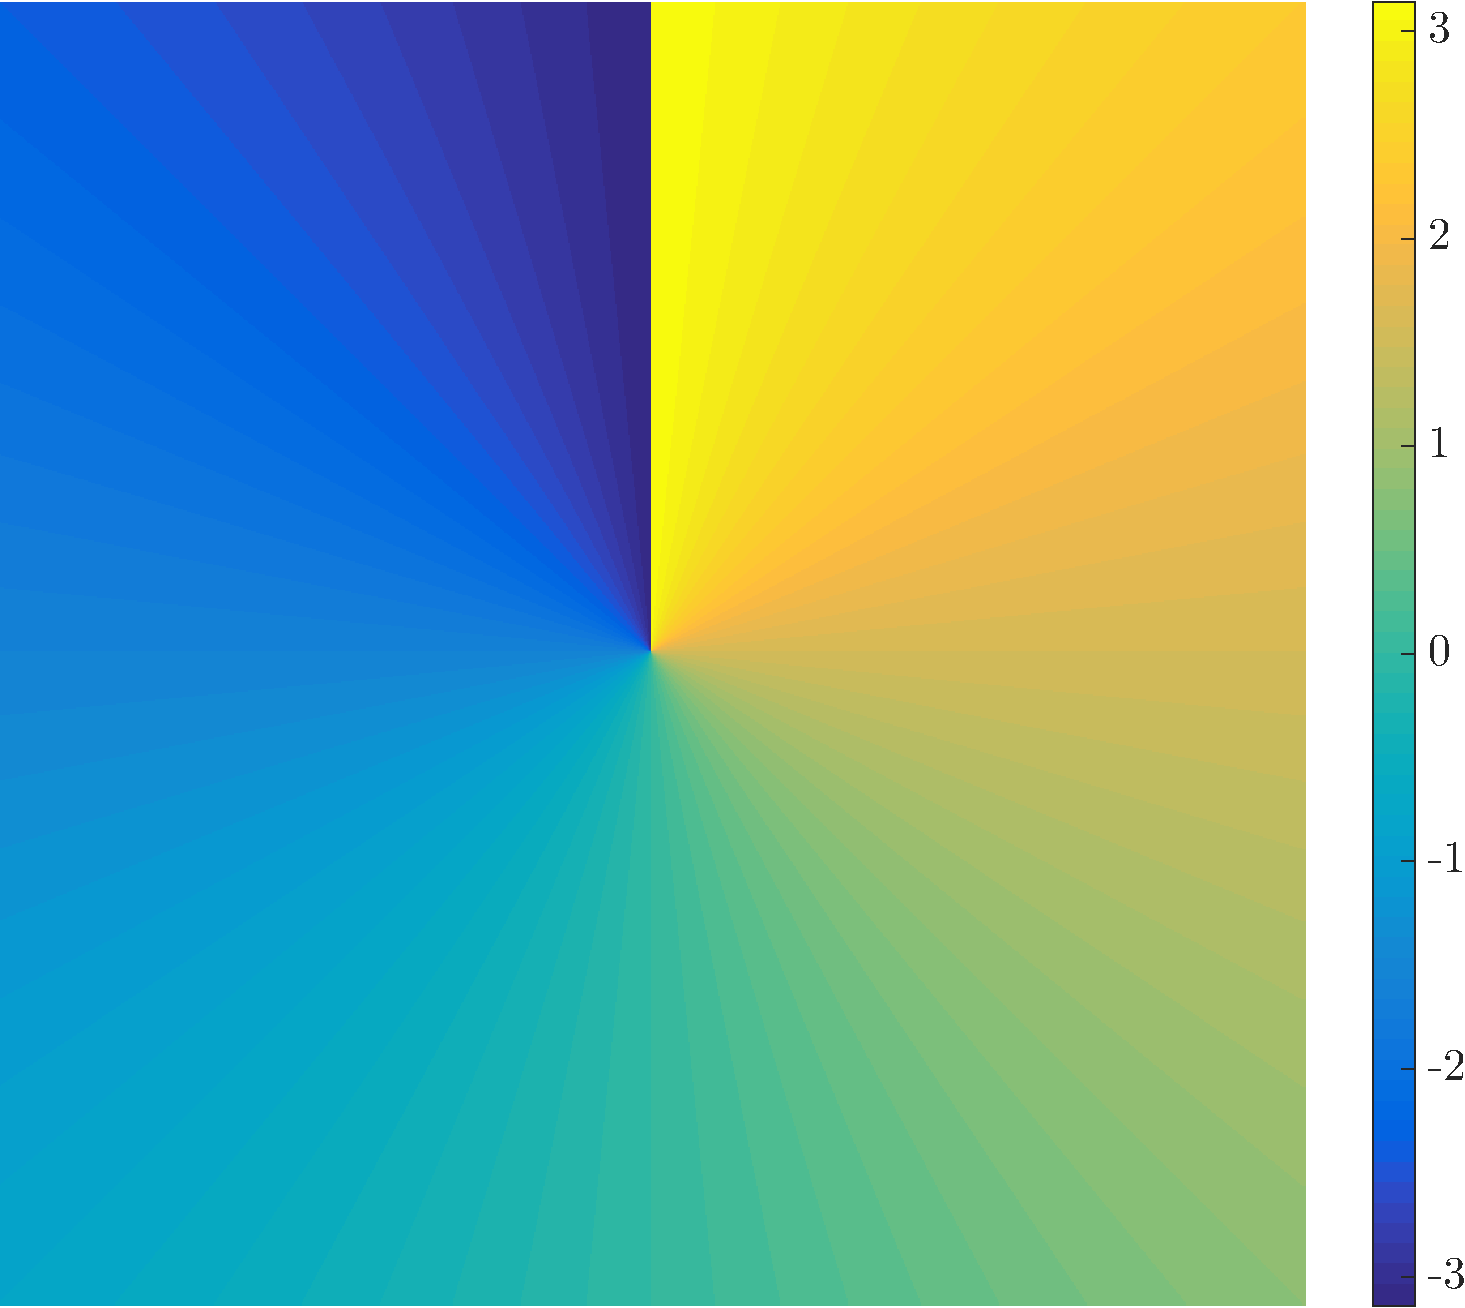
\includegraphics[width=0.45\textwidth]{Images/ch4_vtx/2pi.pdf}
    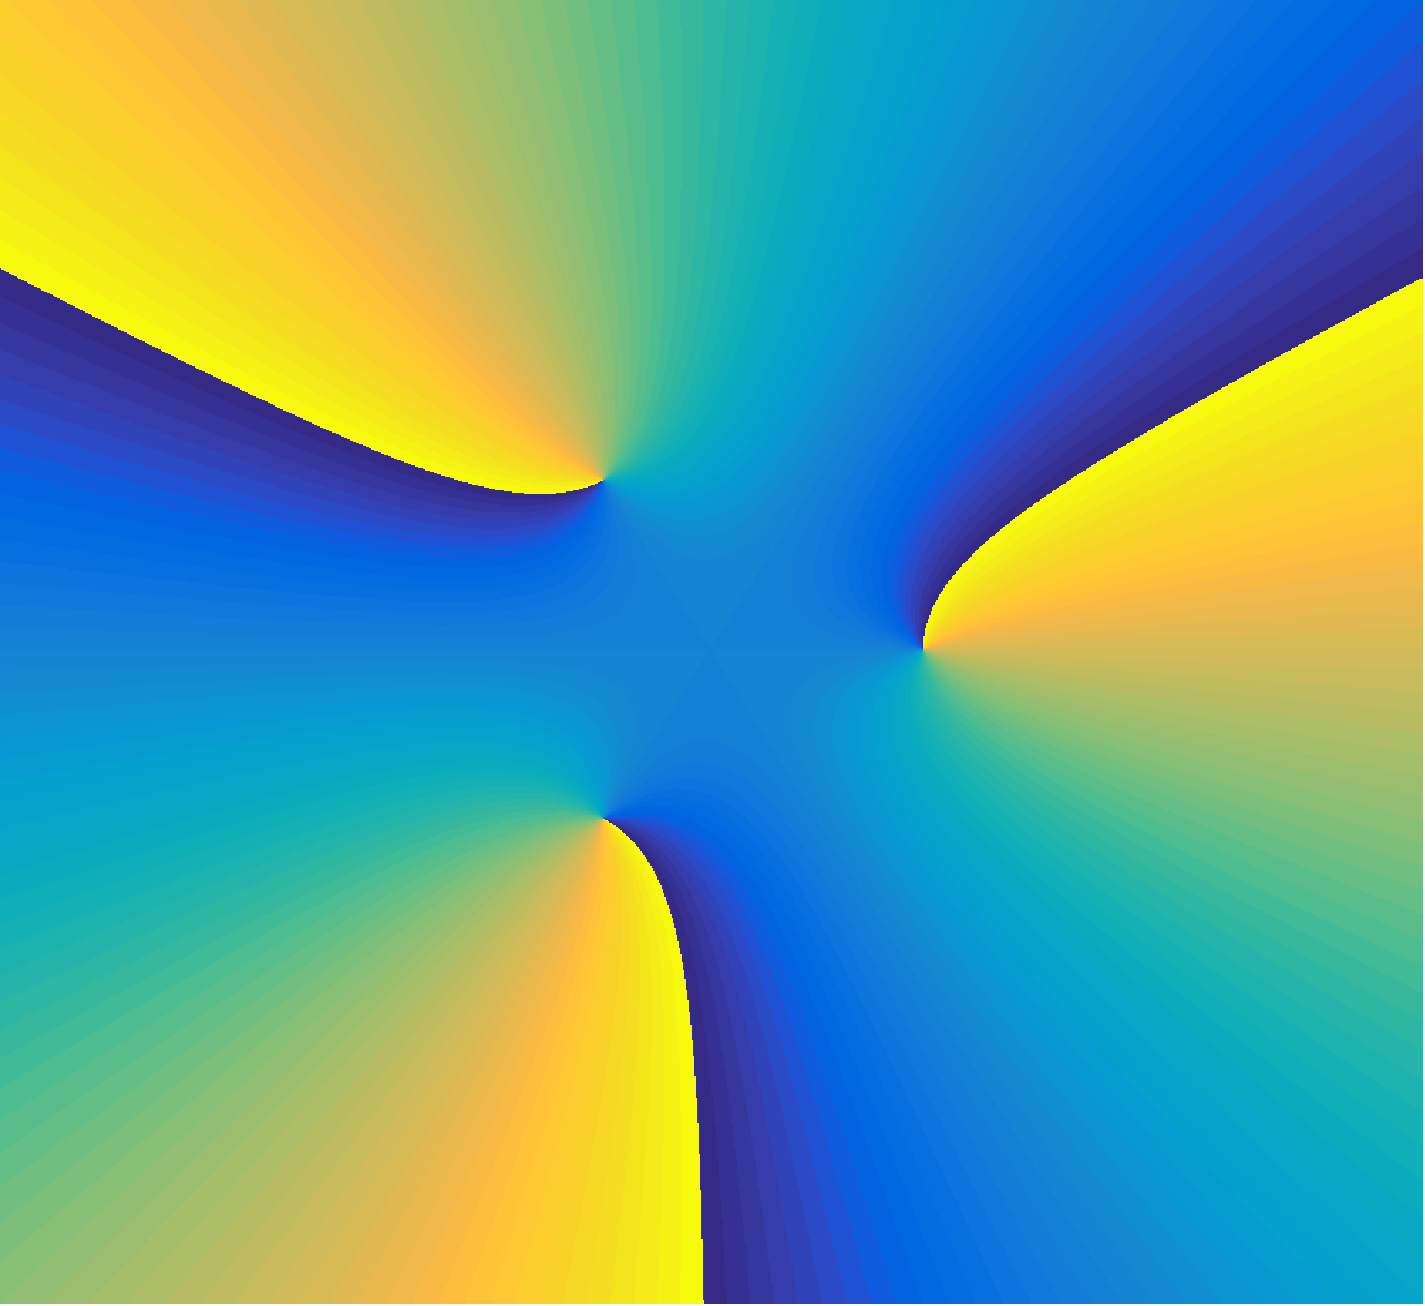
\includegraphics[width=0.435\textwidth]{Images/ch4_vtx/3_2pi.pdf}
    \caption{The $2\pi$ phase winding is shown for a single (L) and three separated (R) defects. The application of separate phase singularities can be treated as summing each individual phase profile, $\left(\displaystyle\sum\limits_i \phi_i \right) \mod 2\pi$.}\label{fig:atan2phase}
\end{figure}


Writing the wavefunction in the standard Madelung transform form, and including the additional phase singularity term $\phi$, I imprint this singularity to the condensate wavefunction as
\begin{equation}
    \Psi(\mathbf{r},t) = |\Psi(\mathbf{r},t)|e^{\text{i}(\theta(\mathbf{r},t) + \phi(\mathbf{r}))}.
\end{equation}
An example of this is given in Fig.~\ref{fig:0to1vtx}, where the condensate density and phase is shown, following imaginary time evolution, before and after a phase imprint.

\begin{figure}\centering
    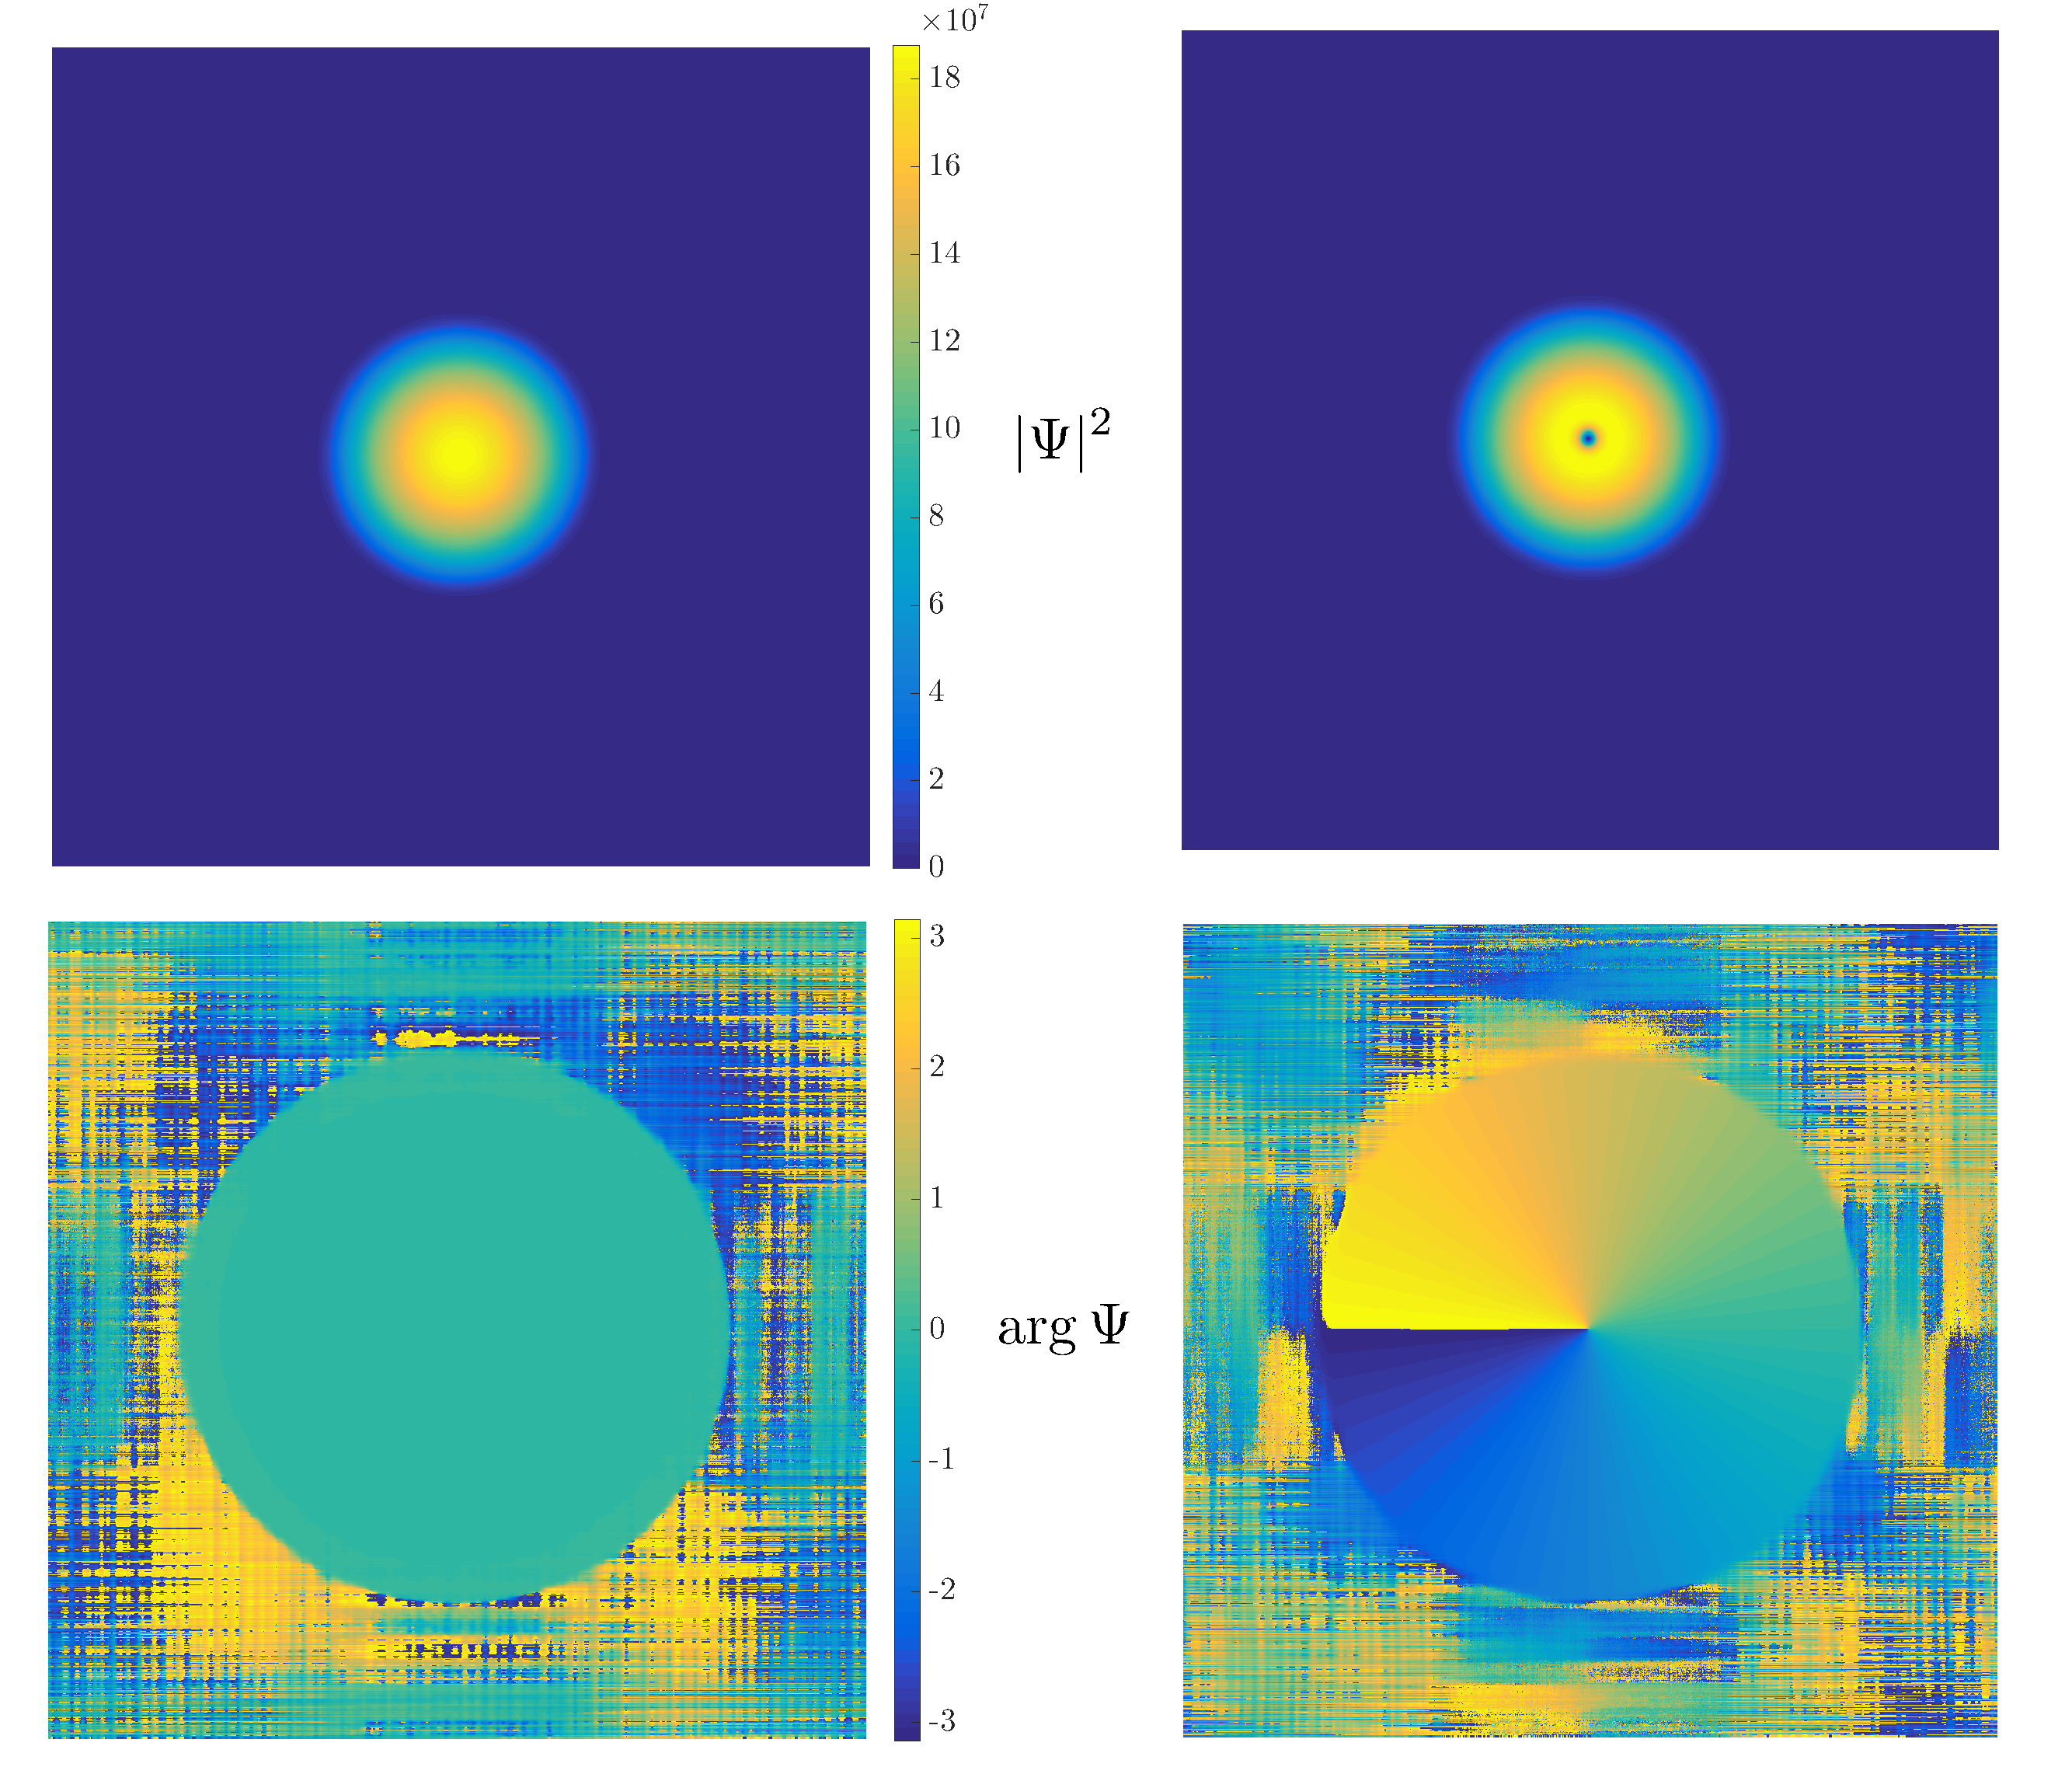
\includegraphics[width=0.75\textwidth]{Images/ch4_vtx/1vtxbec.pdf}
    \caption{The condensate density and phase are shown in the absence and presence of a vortex. The density dip location corresponds exactly with the phase singularity, around which it winds from $-\pi$ to $\pi$}.\label{fig:0to1vtx}
\end{figure}
While here I have shown the creation of a groundstate solution with the phase imprint and imaginary time evolution, this process may also be carried out during real-time evolution. For a closed system the vortex imprint will raise the energy of the system, and likely not be a groundstate. This often rectified by using a phenomenological dissipation parameter. However, since the true nature of this damping is poorly understood, I consider it more instructive to examine the conserved GPE, given the wide variety of success it has shown for modeling condensate dynamics.

\section{Vortex lattice solutions}
Using the vortex imprinting method, the generation of any arbitrary number of vortex-containing condensates is possible, with any required winding. However, as the process of imprinting generates phonons, it can be somewhat difficult to ensure the condensate remains following the imprint of a large number ($10^2$) of imprints. Although, imprinting in imaginary time would alleviate this issue, knowing the actual trap frequency that can stably support $N$ vortices can be tricky. Thus, for the purpose of generating more than a few vortices, evolution in imaginary time at a predetermined rotation frequency $\Omega$ is for my work a preferred method for vortex generation. For a linear ramp of the rotation frequency during imaginary time evolution, as discussed in Sec.~\ref{sec:linramp}, I essentially follow the groundstate solution at all times. This has an added advantage of returning a groundstate solution for any required rotation frequency, with the number of vortices increasing as higher frequencies are reached. An example of several states from a single simulation are given in Fig.~\ref{fig:inc_omega}. The previously discussed resolution considerations become apparent as the rotation rate is increased for both position and momentum space representations of the wavefunction. A sample movie of the generation is given here \cite{MLXD:movie_groundstates}, wherein I ramp the frequency from $\Omega/\omega_\perp = 0.39 \to 0.995$ and plot the density in position space.

\begin{figure}\centering
    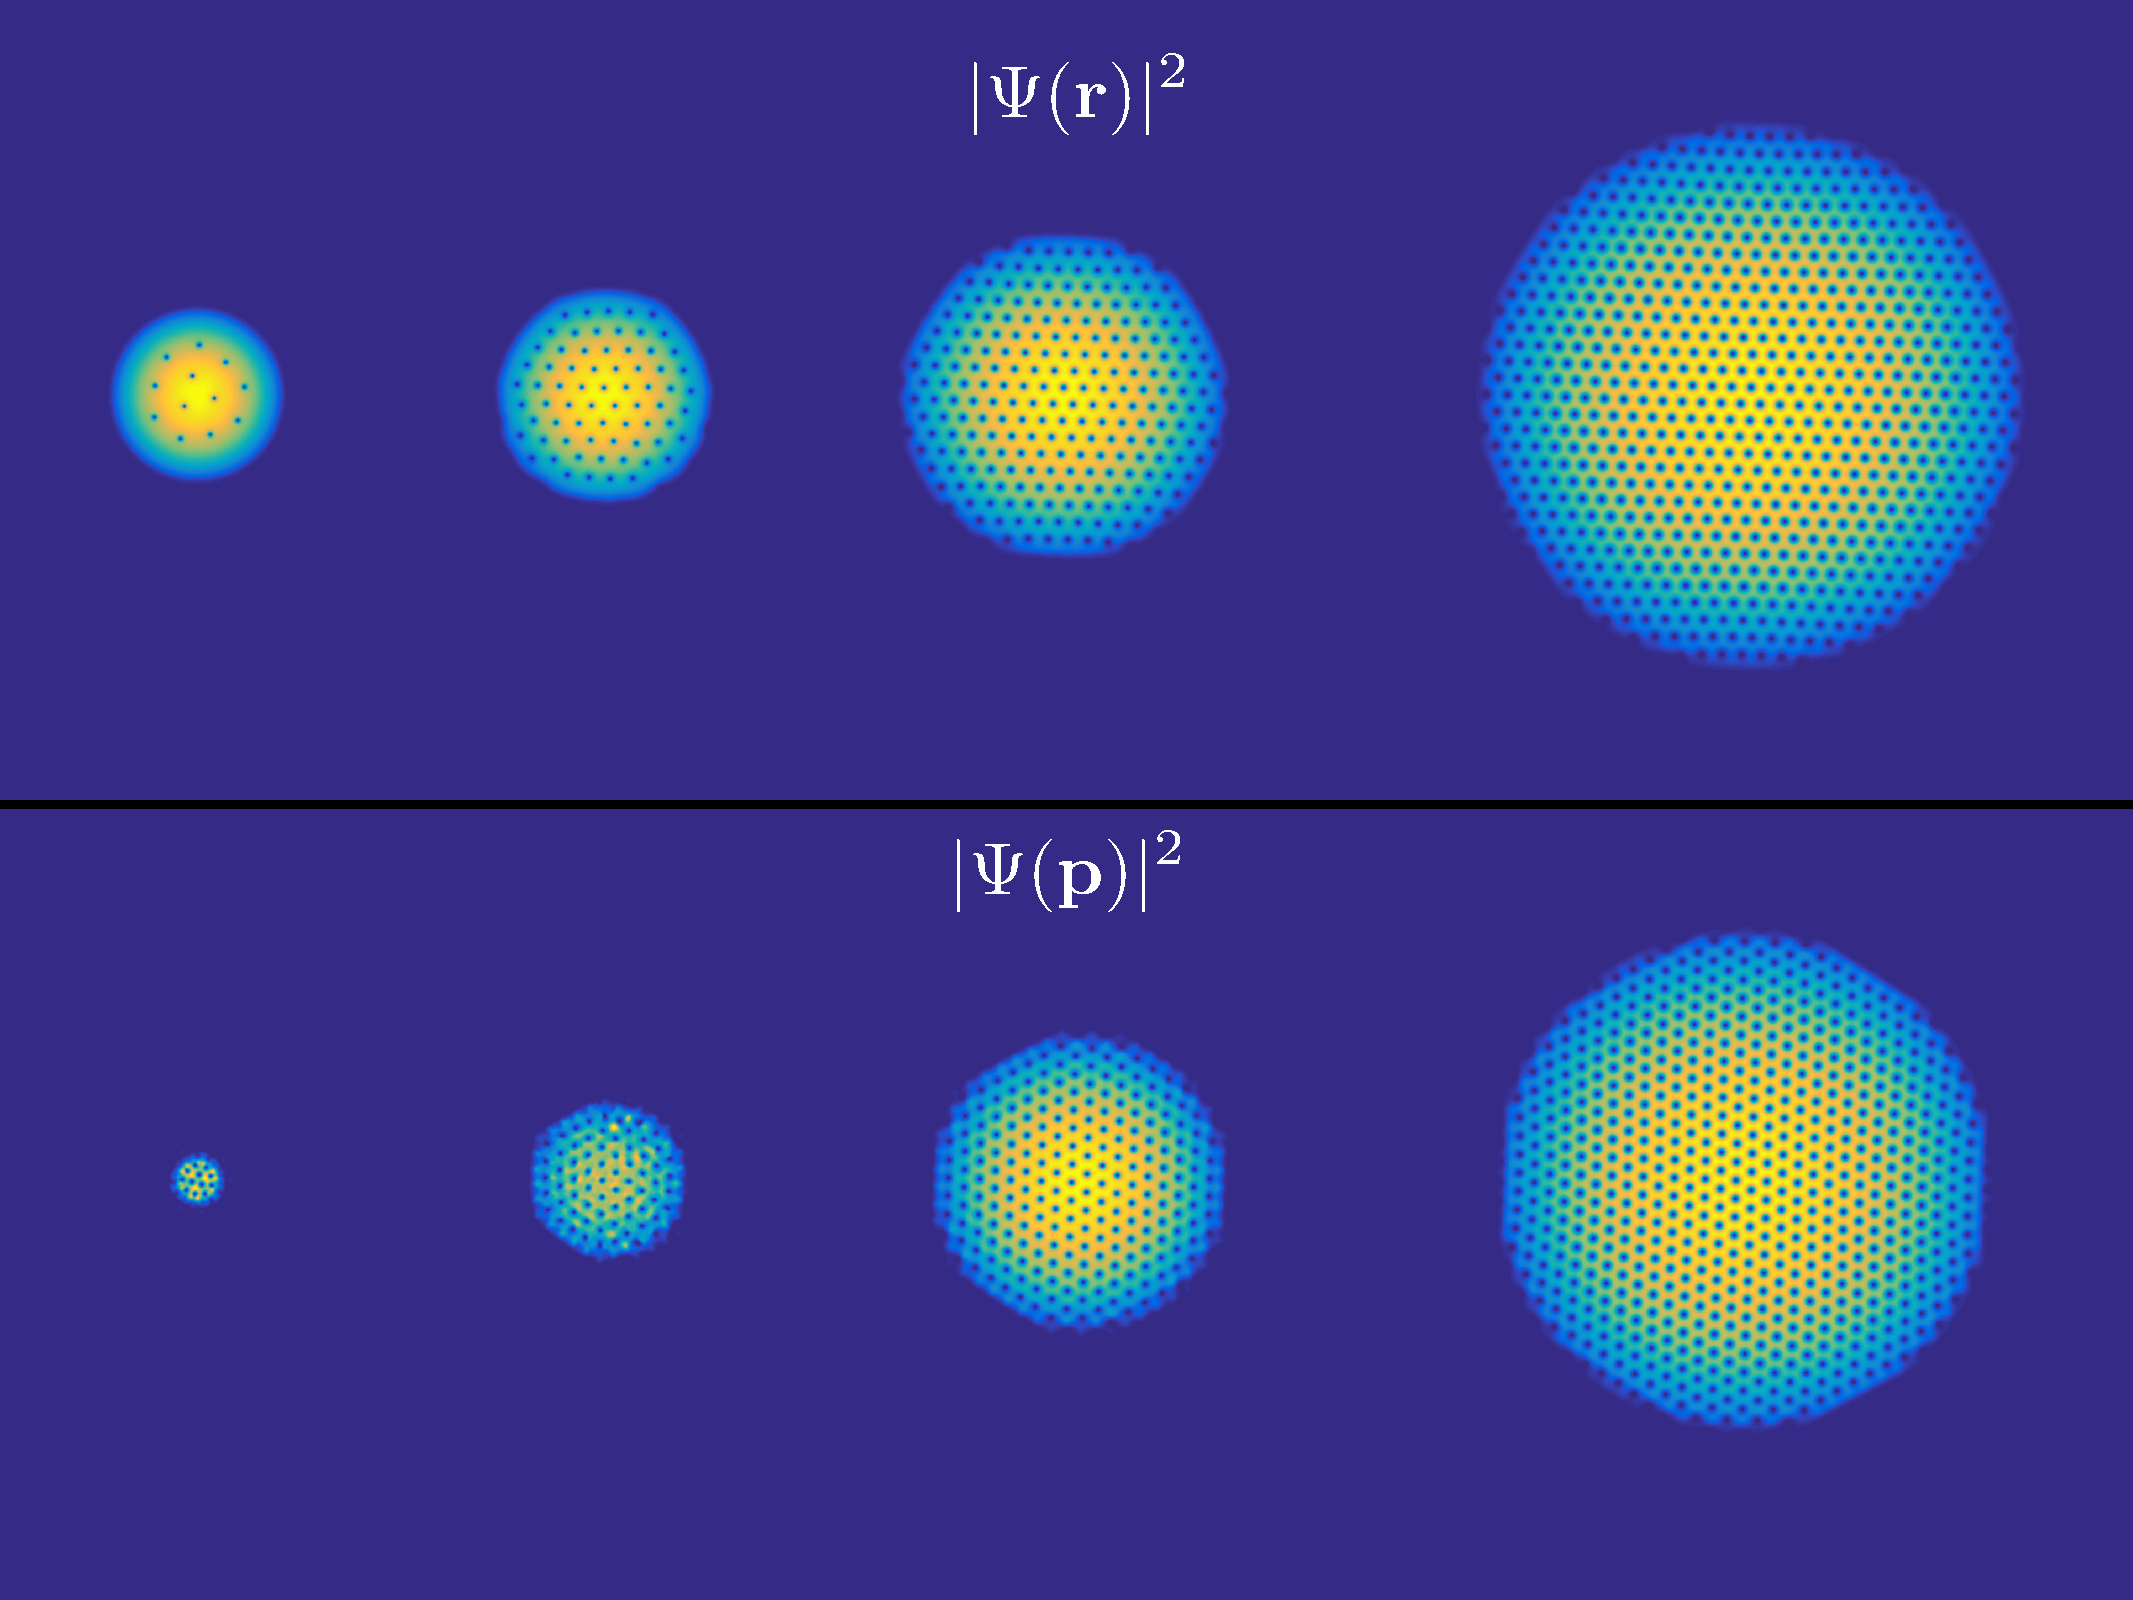
\includegraphics[width=0.85\textwidth]{Images/ch4_vtx/ramp_omega.pdf}
    \caption{The density distributions of the wavefunction in position (top) and momentum (bottom) space are given for rotation frequencies (L-R) $\Omega/\omega_\perp=[0.366,0.796,0.962,0.995]$. The color axis differs for each plot, as a constant axis is difficult to view densities across all magnitudes. The growth rate of the condensate radius in both position and momentum space becomes large when $\Omega \approx \omega_\perp$.}
    \label{fig:inc_omega}
\end{figure}

If the linear ramp is performed too quickly, or if I instantaneously choose a groundstate with a large amount of angular momentum, the vortices tend to enter from the boundary all at one instance, and fail to ever find a well ordered groundstate. An example of this such issue is given by Fig.~\ref{}, and indicates the need for a slow linear ramp that is essentially adiabatic in imaginary time.
\begin{figure}
    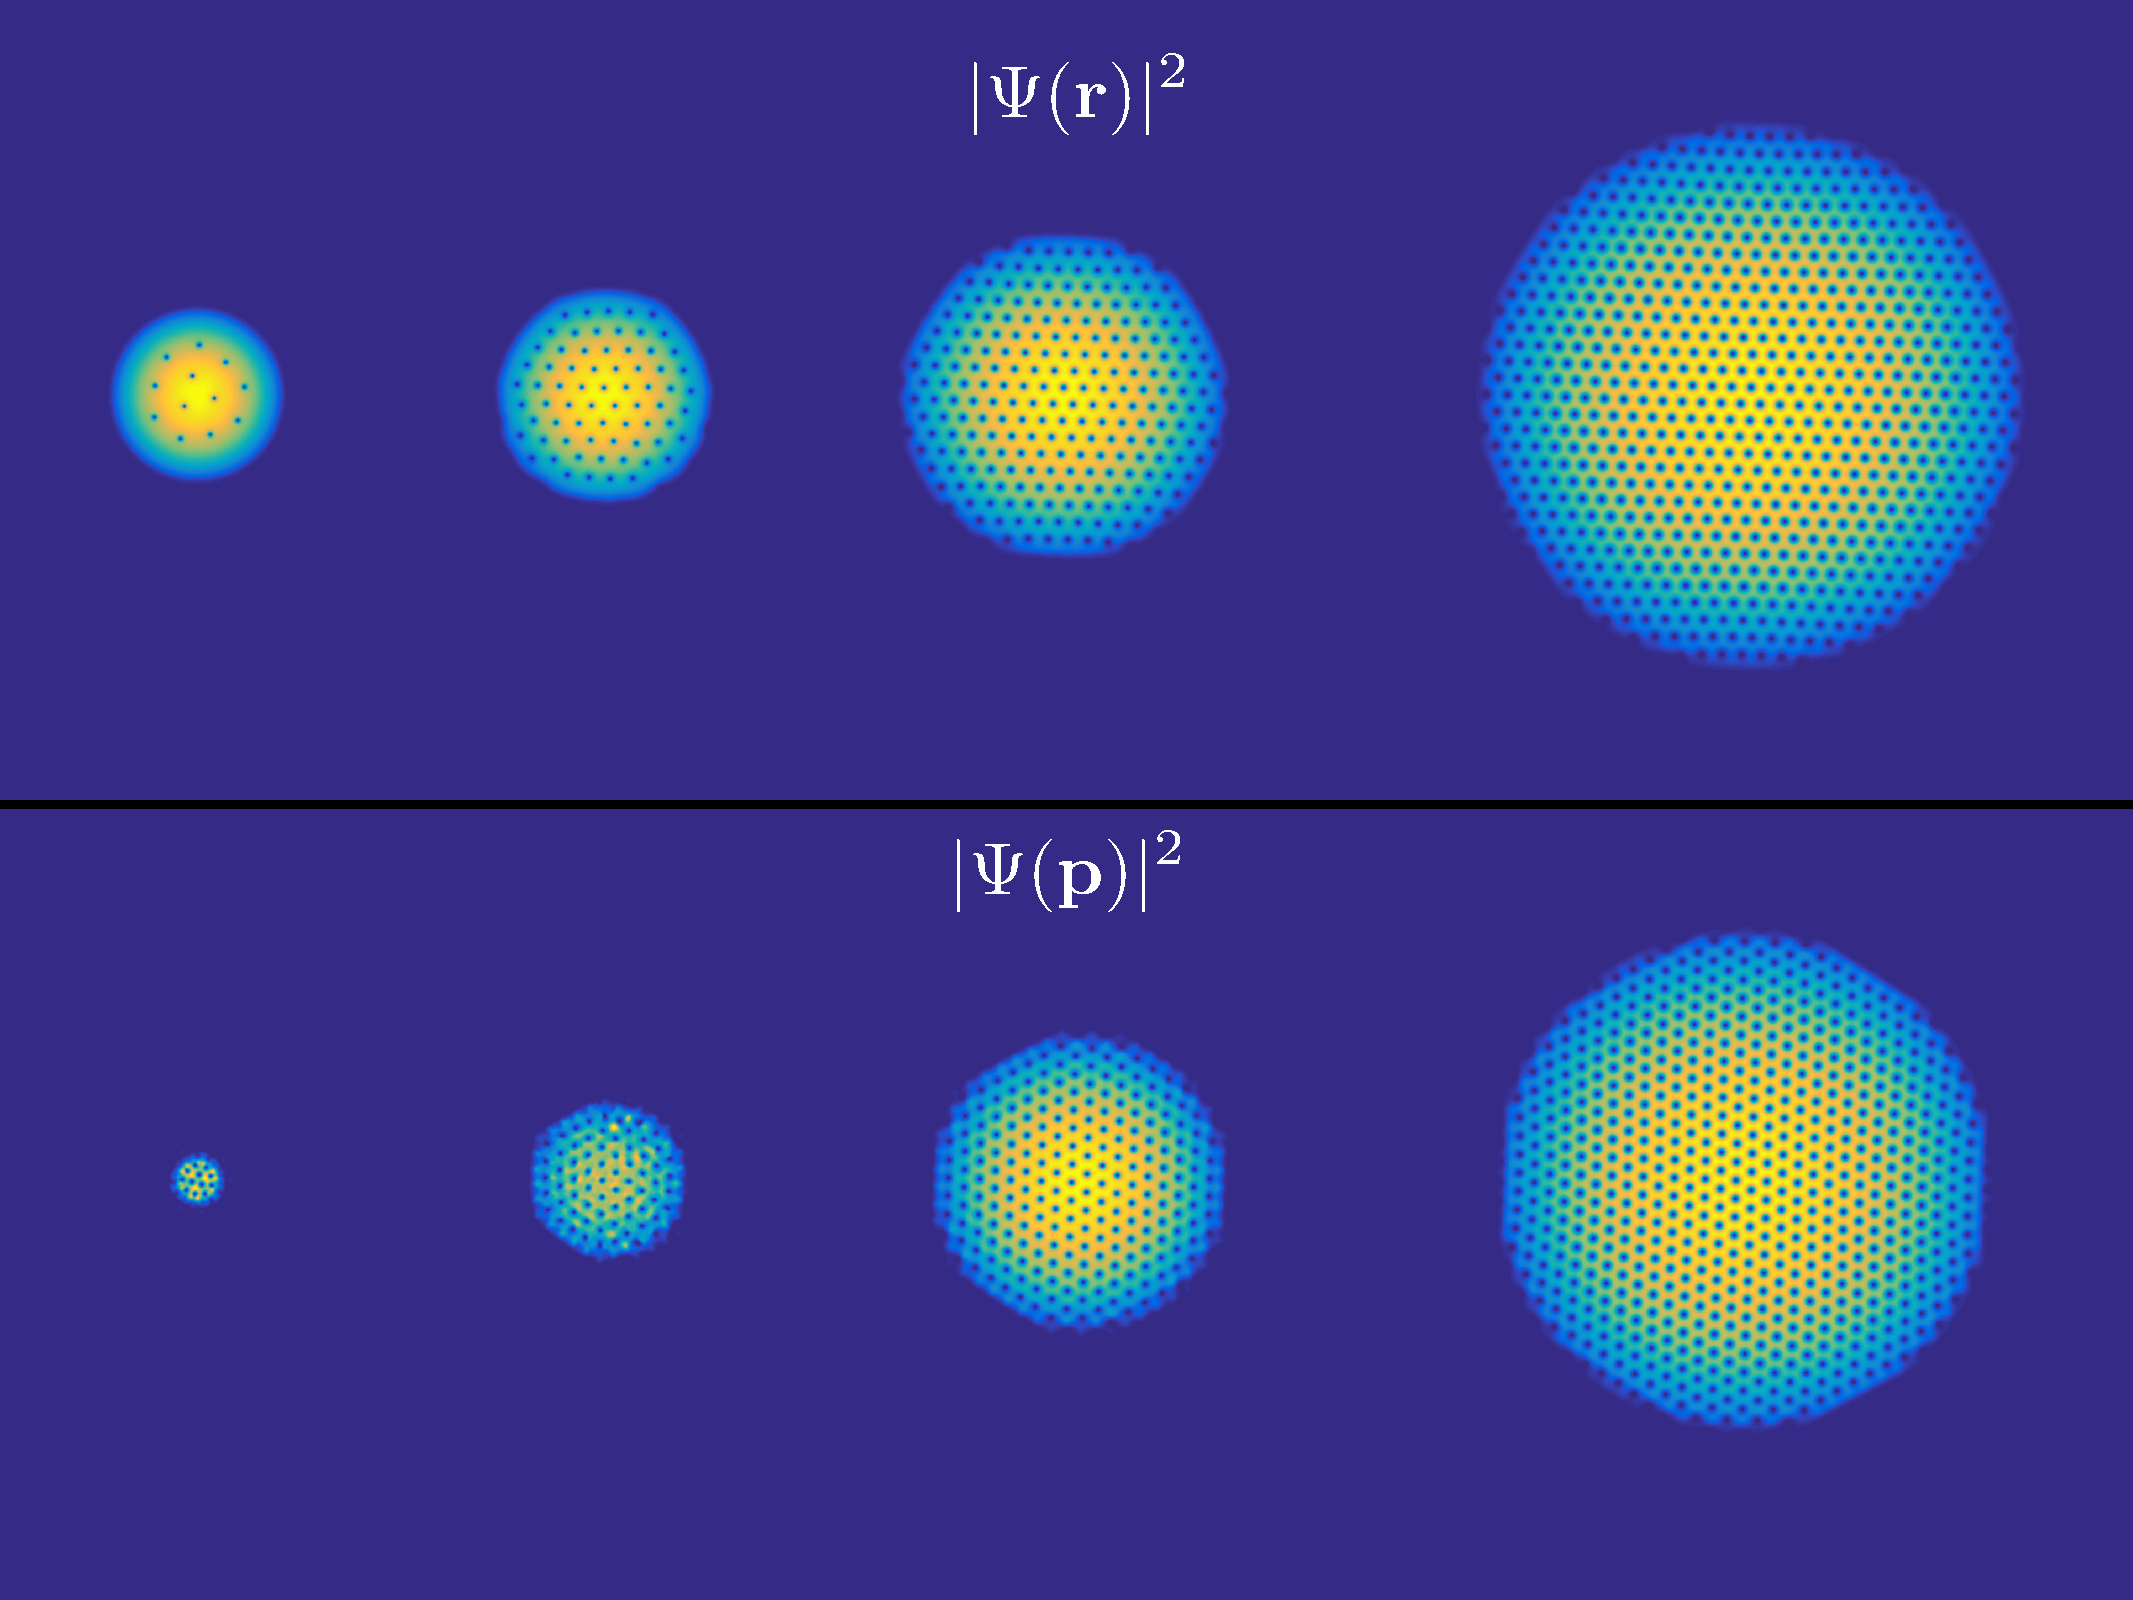
\includegraphics[width=0.85\textwidth]{Images/ch4_vtx/ramp_omega.pdf}
    \caption{The density distributions of the wavefunction in position (top) and momentum (bottom) space are given for rotation frequencies (L-R) $\Omega/\omega_\perp=[0.366,0.796,0.962,0.995]$. The color axis differs for each plot, as a constant axis is difficult to view densities across all magnitudes. The growth rate of the condensate radius in both position and momentum space becomes large when $\Omega \approx \omega_\perp$.}
    \label{fig:malformed_lattice}
\end{figure}

\section{Rapidly rotating vortex lattice}
Given the need for a well ordered vortex lattice it is instructive to discuss the generation of such a system. I assume an initial wavefunction guess of a two-dimensional gaussian having some finite overlap with the groundstate of the system in the absence of angular rotation. Following an imaginary time-evolution like what was outlined in Sec.~\ref{sec:numerics}, the groundstate of the condensate is found.


\subsection{Gaussian phase}

\subsubsection{One dimensional}

\subsubsection{Two dimensional}



\section{Few vortex states}
As discussed in Section~\ref{sec:superfluid}, the discovery and manipulation of quantum vortices remains an active area of research.


Given that the energy of a vortex-carrying condensate scales as $E\propto l^2$, as $L_z \propto l$, any increase in the angular momentum causes a squared increase in the energy. Thus, for energetic favorability, the system prefers to maintain singly-charged vortices. To generate a vortex in the condensate costs energy,

Wi

\section{Quantum vortex dynamics}



\section{Vortex lattice states}
    \begin{equation}
        E(\Psi) = \int \Psi^{*} H_{\text GP} -\Omega L_z \Psi
    \end{equation}
